\mode<all>
% Incluyo los paquetes necesarios.
% para no tener problemas con acentos etc.
\usepackage[utf8]{inputenc}
% en español
\usepackage[spanish]{babel}
%matemática
\usepackage{amsmath}
% este no se si hace falta pero por las dudas
\usepackage{graphicx}
% para incluir peliculas
\usepackage{multimedia}
% para usar segunda pantalla
\usepackage{pgfpages}
\usepackage{pgf}
% para hacer dibujitos
\usepackage{tikz}
\usetikzlibrary[automata,calc,arrows,decorations.pathmorphing,backgrounds,shapes,
patterns,positioning,fit,petri,overlay-beamer-styles]
\tikzstyle{every picture}+=[remember picture]
%recuadros sencillos
%\usepackage{tcolorbox}
% enumeradores intercambiables
\usepackage{enumerate}
% para subtitulos en figuras
\usepackage{subcaption}
%listings for code input
\usepackage{listings}
%verbatim input from file!
\usepackage{verbatim}
\usepackage{fancyvrb}
% para modificar los encabezados y pies de página.
%\usepackage{fancyhdr}
%\pagestyle{fancy}
\usepackage{standalone}

\definecolor{codegreen}{rgb}{0,0.6,0}
\definecolor{codegray}{rgb}{0.5,0.5,0.5}
\definecolor{codepurple}{rgb}{0.58,0,0.82}
\definecolor{backcolour}{rgb}{0.95,0.95,0.92}

\lstdefinestyle{codeblock}{
    backgroundcolor=\color{backcolour},   
    commentstyle=\color{codegreen},
    keywordstyle=\color{magenta},
    numberstyle=\tiny\color{codegray},
    stringstyle=\color{codepurple},
    basicstyle=\ttfamily\footnotesize,
    breakatwhitespace=false,         
    breaklines=true,                 
    captionpos=b,                    
    keepspaces=true,                 
    numbers=left,                    
    numbersep=5pt,                  
    showspaces=false,                
    showstringspaces=false,
    showtabs=false,                  
    tabsize=2
}


%\mode<presentation>{
% para ver las notas con la presentacion.  
%\setbeameroption{hide notes}
%para dejar las notas en la segunda patnalla
%}

% incluyo los beamercolors
\include{./PREAMBLE/BEAMERCOLORS}

%incluyo el tema y modificaciones
\include{./PREAMBLE/BEAMERTHEME}

% modifico los temas
\include{./PREAMBLE/THEMES}
% defino el template para la diapositiva del título

%%%%%%%%%%%%%%%%%%%%%%%%%%%%%%%%
% Defino la Clase
%%%%%%%%%%%%%%%%%%%%%%%%%%%%%%%%
\subtitle[Modelización 2020]{ Modelización de Propiedades y Procesos 2020 }
\author{
  Ruben Weht\inst{1,2} 
  \and Silvio Terlisky\inst{1,3}
  \and Pablo Gargano\inst{1,3} 
  \and Mariano Forti\inst{1,3} 
}
\institute{
  \inst{1}Instituto de Tecnología Prof. Jorge Sabato
  \and
  \inst{2}Fisica del Sólido, Edificio TANDAR,
  \and
  \inst{3} Gerencia Materiales
}

\mode<presentation>{\date{\scriptsize\href{mailto:model.sabato@gmail.com}{model.sabato@gmail.com}}}

\mode<article>{
  \date{
    \small
  \textsuperscript{1}Instituto de Tecnología Prof. Jorge Sabato\\
  \textsuperscript{2}Fisica del Sólido\\
  \textsuperscript{3}Gerencia Materiales\\
  \href{mailto:model.sabato@gmail.com}{model.sabato@gmail.com}
}

%defino los encabezados y pies de págna para
% dodo el documento en función de la materia y la
% clase.
%\fancyhead[L]{\tiny Modelización de Materiales 2019}
%\fancyhead[R]{\tiny \leftmark}
}

\title{
  \mode<article>{
\includegraphics[height=1cm]{./PREAMBLE/logo-isabt25.png}
\hfill
\includegraphics[height=1cm]{./PREAMBLE/ISOLOGOCNEA.png}
\hfill
\includegraphics[height=1cm]{./PREAMBLE/logo-unsam.png}
\\}  Formato Gmsh}
\subject{Introducción al formato de Gmsh}
\keywords{Matlab, Modelizacion 2019, Programación,gmsh}
% Inicia el documento.
\begin{document}

% Título de la clase. 
\mode<presentation>{
\begin{frame}[plain]
\titlepage
\end{frame}
}

\mode<article>{
\maketitle
}


\mode<all>

\section{Nuevas Herramientas}
\input{./01-NuevasHerramientas/01-01-NE}
\mode<article>
\subsection{Uso de herramientas}

Recuerde que todo problema puede separarse en las etapas de 
Preproceso, proceso y Post Proceso. Hasta ahora las únicas 
herramientas usadas fueron papel y lápiz para el pre-proces
y su lenguaje de programación para el Proceso y Post Proceso. 
A partir de ahora se suma la necesidad de usar un software
que nos permita generar los mallados (matriz de nodos y de 
conectividad) ya que la cantidad de elementos y nodos será 
arbitraria para cualquiera de los problemas. Utilizaremos
Gmsh para las etapas de Preproceso y Post Proceso.

Esto implica que deberemos ser capaces de generar la 
comunicación entre nuestro programa de proceso o solver
y la herramienta de pre y post proceso. Con ese 
fin utilizaremos arhivos de texto plano con formato. 
Por lo tanto es necesario que recuerde las sentencias para
lectura y escritura de archivos, introducidas anteriormente en
la Clase Práctica de Introducción a la Programación. Este 
concepto se esquematiza en la \ref{FiguraComunicarHerramientas}
Nuestro programa solver Deberá ser capaz de leer las 
matrices de conectividad y de nodos de las mallas generadas
por Gmsh, y de escribir los resultados en un formato que 
pueda ser usado en esta útlima herramienta para visualizarlos.
Estas relaciones se esquematizan en la Figura 
\ref{FiguraFlujoTrabajo} .
Nuestro Mallador generará la matriz de nodos y 
  la matriz de conectividad a partir de una geometría 
  arbitraria. Toda la información se guarda en archivos 
  de texto que deberemos poder escribir y leer .




\begin{figure}
  \includeslide[width=\textwidth]{FrameComunicarHerramientas}
  \caption{Escquema de la relación entre las herramientas 
  usadas. Usaremos Archivos de texto plano para intercambiar
  información. \label{FiguraComunicarHerramientas} }

\end{figure}

\begin{figure}
  \includeslide[width=\textwidth]{FrameFlujoTrabajo}
  \caption{ Ejemplo del Puente con la Geometría y
  matrices de conectividad y nodos dadas por Gmsh.
  \label{FiguraFlujoTrabajo}
  }
\end{figure}

\mode*
\begin{frame}<presentation>[label=FrameUsoHerramientas]
  \frametitle{Uso De Herramientas}
  \includegraphics[width=\textwidth,page=3,bb=0cm 1cm 28cm 16cm,clip]{./GMSH_fileformat_2019.pdf}
\end{frame}

\begin{frame}<presentation>[label=FrameComunicarHerramientas]
  \frametitle{Comunicación entre Herramientas}
  \includegraphics[width=\textwidth,page=4,bb=0cm 1cm 28cm 16cm,clip]{./GMSH_fileformat_2019.pdf}
\end{frame}

\begin{frame}<presentation>[label=FrameFlujoTrabajo]
  \frametitle{Flujo de trabajo}
  \includegraphics[width=\textwidth,page=5,bb=0cm 1cm 28cm 16cm,clip]{./GMSH_fileformat_2019.pdf}

\end{frame}
\mode<all>


\section{Definición de Mallados}
\subsection{Geometrías}
\mode<article>

Las geometrías pueden definirse en archivos de texto plano con
extensión \texttt{.geo}. Estos archivos de geometría pueden
contener elementos de programación generales. Como se
esquematiza en la Figura \ref{FiguraEjemploGeometrias} 
es posible hacer comentarios y definir variables. La geometría
se genera mediante instrucciones con sintaxis específica. 

Debe tenerse en cuenta que la construcción de geometrías 
complejas es jerárquica. Por ejemplo, para definir un 
rectángulo deben definirse primero sus vértices, luego 
los lados, luego el borde (el lazo que contiene la superficie) y
por último su superficie. En las versiones más nuevas de gmsh
se han incluido instrucciones para definir estructuras complejas
en pocas instrucciones pero la estructura final de la 
matriz de conectividad refleja siempre estas estructuras jerárquicas. 
Las instrucciones siempre se terminan con un punto y coma (\texttt{;}).

\subsubsection{Factores de escala}
La definición de los puntos se realiza mediante la instrucción 

$$ Points( i ) = { x_i, y_i , z_i , fe } ; $$

donde los tres primeros valores corresponden a las coordenadas
cartesianas del punto, y el cuarto valor corresponde al 
\emph{factor de escala}. Este número será de gran utilidad
en el momento de mallar los recintos de integración, i.e. al 
generar los elementos finitos que aproximan el recinto de interés. 
El valor del factor de escala corresponde con el tamaño 
característico de los elementos finitos alrededor del punto
definido. Por lo tanto, en un punto donde se necesita 
mayor resolución se puede usar un factor de escala pequeño,
mientras que en un punto donde no se requiere gran resolución
puede usarse un factor de escala grande. Los valores 
concretos dependen del tamaño característico en la geometría 
del problema en resolución. 

\begin{figure}
  \includeslide[width=\textwidth]{FrameEjemplosGeometrias}
  \caption{Generalidades del formato para escribir geometrías
  \label{FiguraEjemploGeometrias}
  }

\end{figure}

\mode*
\begin{frame}<presentation>[label=FrameEjemplosGeometrias]
  \frametitle{Geometrías}

  \begin{columns}

    \column{0.3\textwidth}
      \begin{codeblock}
	\scriptsize{
      \verbatiminput{./Ejemplos/chapa-clase.geo}
    }
    \end{codeblock}
    \column{0.7\textwidth}
    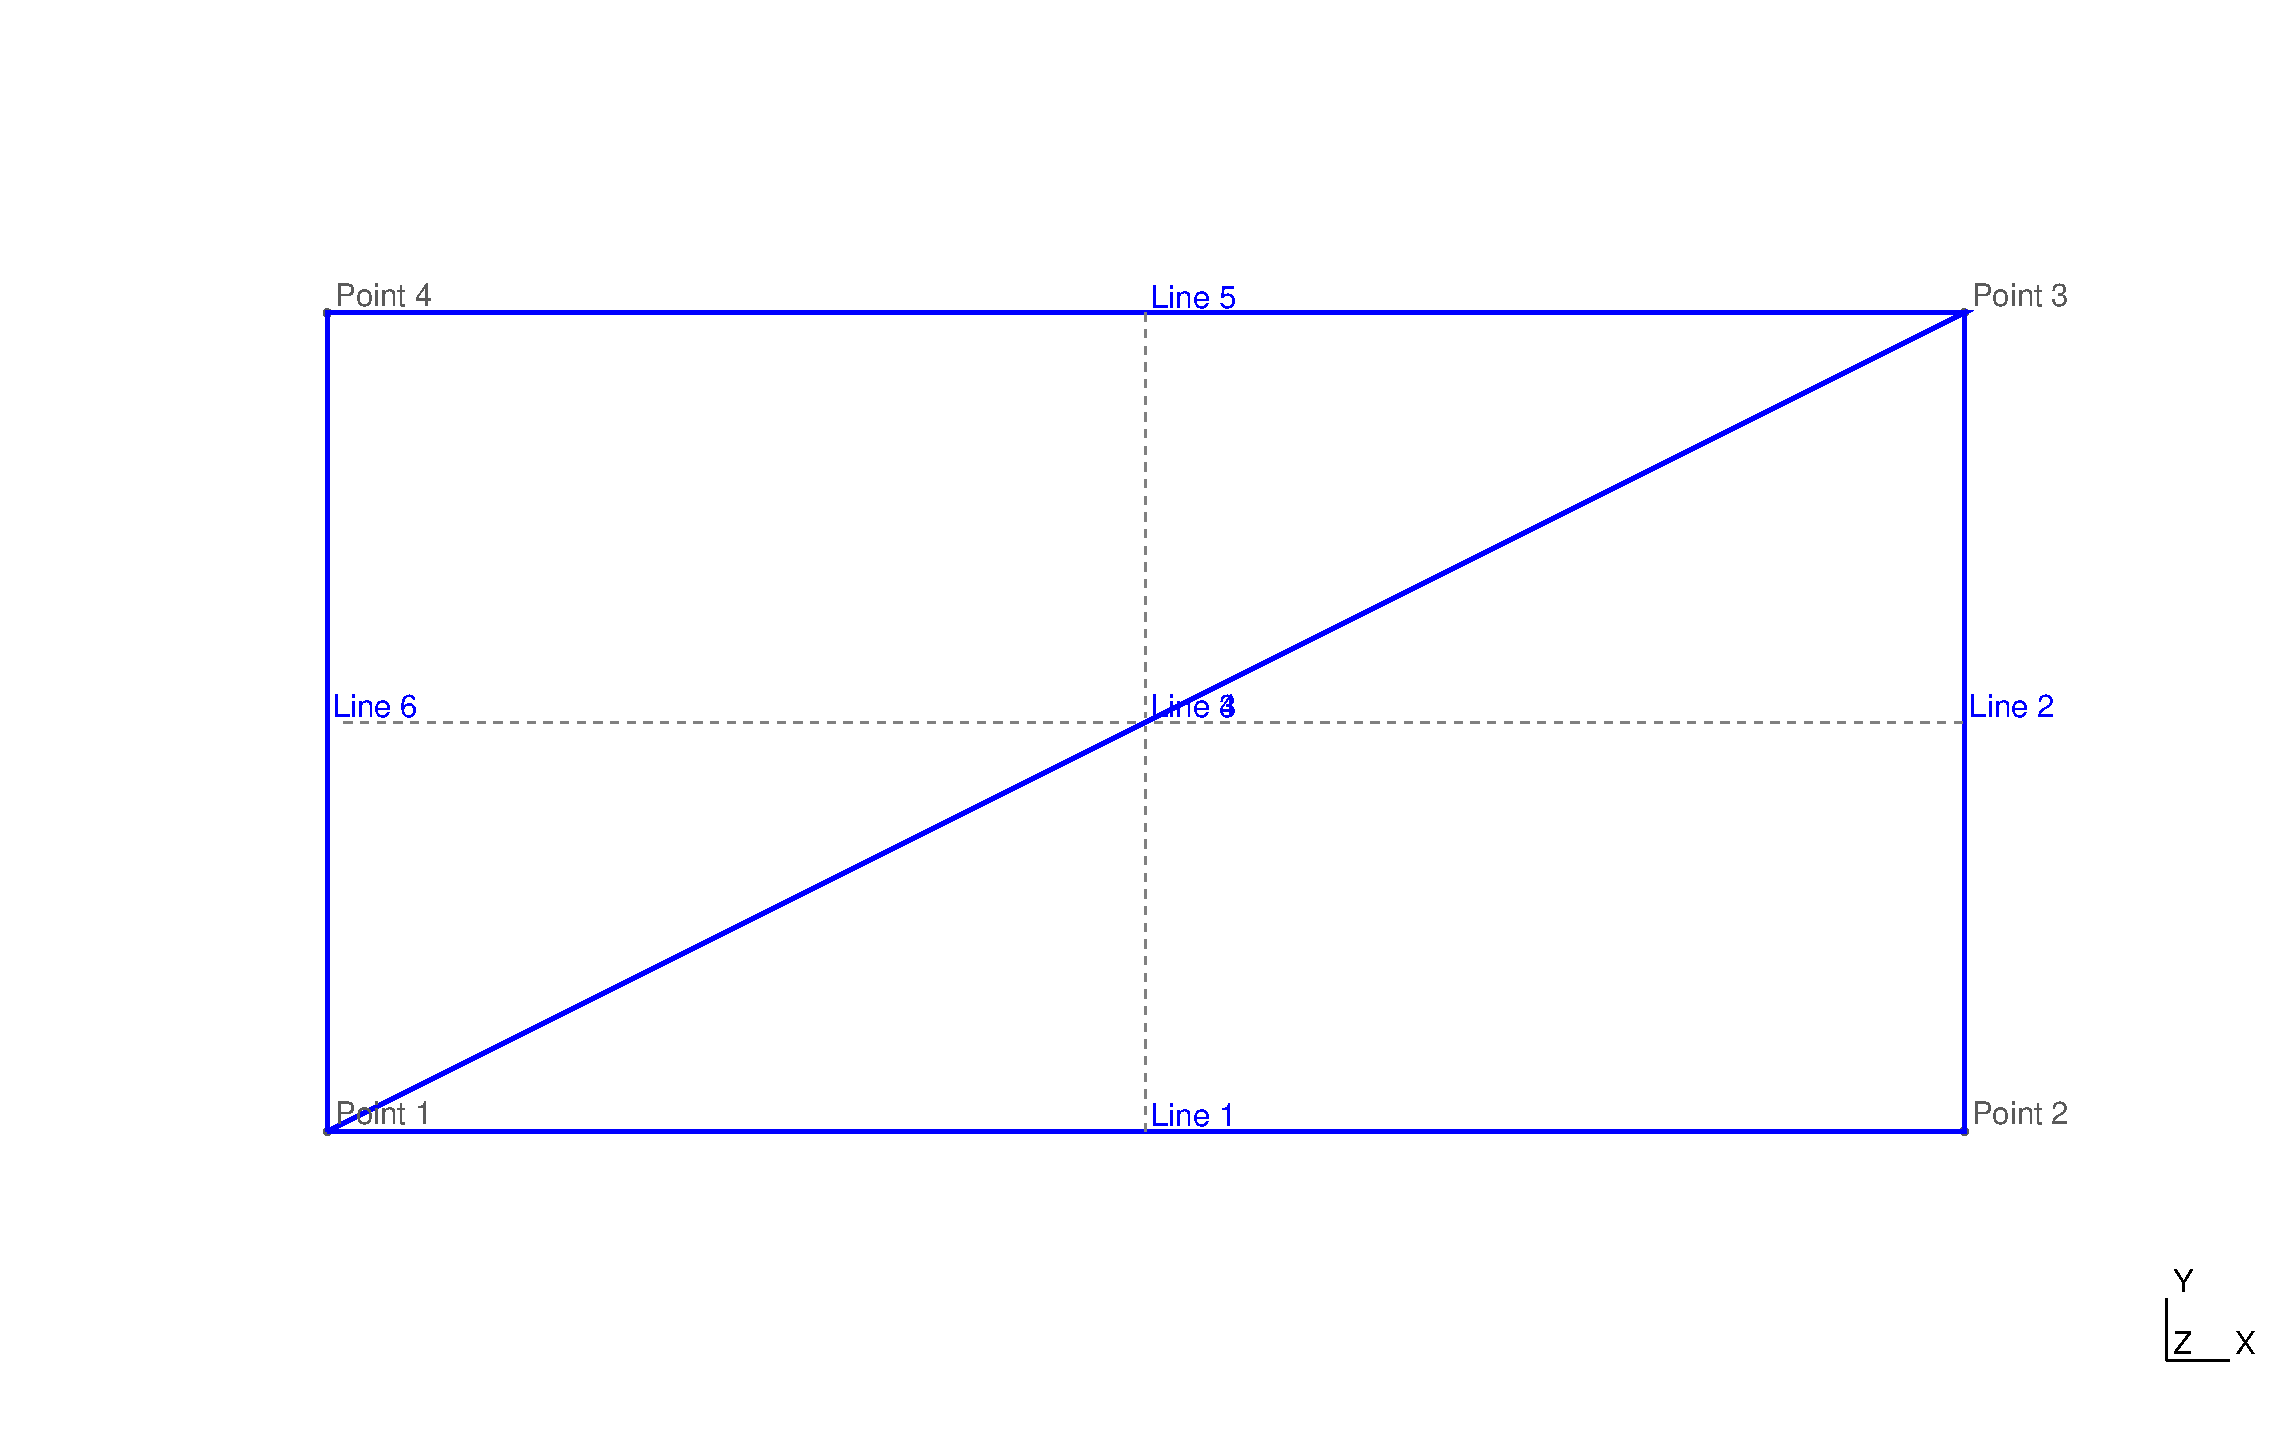
\includegraphics[width=\textwidth]{./Ejemplos/PuenteClase.pdf}
  \end{columns}


%  \includegraphics[width=\textwidth,page=6,bb=0cm 1cm 28cm 16cm,clip]{./Libreoffice/GMSH_fileformat.pdf}

\end{frame}

\mode<all>

\subsection{Mallados}
\mode<article>
Los Archivos de definición de los mallados se guardan en 
archivos de texto plano con extensión 
\texttt{.msh}. Son un poco más 
complejos. Como se esquematiza en la Figura 
\ref{FiguraEstructuraMallados} puede separarse su estructura
en bloques. 
\begin{figure}
  \includeslide[width=\textwidth]{FrameEstructuraMallados}
  \caption{Esquema de la etructura en bloques del archivo
  de mallados\label{FiguraEstructuraMallados} }
\end{figure}

\subsubsection{Encabezado}

El encabezado del archivo de mallado indica la versión del 
interprete de mallados que gmsh debe usar. Tómelo como
una receta. 

\subsubsection{Definición de Matriz de Nodos}

Inmediatamente después del encabezado sigue el bloque de 
la definición de los nodos. Como se esquematiza en la 
Figura \ref{FiguraEncabezado} las etiquetas \texttt{\$Nodes} 
y \texttt{\$EndNodes} encierran la definición de los 
nodos. Primero debe indicarse el número de nodos 
presentes. Luego se definen los nodos con su índice y sus 
coordenadas cartesianas. Siempre se indican tres coordenadas. 

\begin{figure}
  \includeslide[width=\textwidth]{FrameEncabezado}
  \caption{ Esquema de los bloques de encabezado y de 
  definición de Nodos \label{FiguraEncabezado} }

\end{figure}

\subsubsection{Definición de Elementos}

Luego del bloque de nodos debe seguir el bloque de los 
elementos, que se delimita por las etiquetas 
\texttt{\$Elements} y \texttt{\$EndElements} como se 
esquematiza en la Figura \ref{FiguraDefinicionElementos}. En
primera instancia debe indicarse el número total de elementos 
a considerar. Debe notarse que s posible tomar definiciones
de elementos de disntinas naturalezas. De hecho, al guardar
un mallado cualquiera desde la interfaz de gmsh puede 
encontrarse que los puntos, líneas y demas elementos 
geométricos de menor gerarquía forman elementos en 
el archivo. Por esta razón se indica luego del numero de
elemento (columna 1) el \texttt{tipo} de elemento. La
codificación para el tipo de elemento puede encotrarse 
en el manual de gmsh. 

Luego del tipo de elemento, debe indicarse el número de 
etiquetas descriptivas que siguen. estas etiquetas indican
pertenencia  a elementos geométricos de mayor gerarquía 
(por ejemplo superficies). En los archivos
que han sido guardados en gmsh se guardan siempre dos 
etiquetas. 

Luego de las etiquetas sigue la matriz de conectividad para 
el elemento de la fila en tratamiento.

\begin{figure}
  \includeslide[width=\textwidth]{FrameDefinicionElementos}
  \caption{Esqema del contenido del bloque de elementos
  \label{FiguraDefinicionElementos} }
  
\end{figure}

\mode*

\begin{frame}<presentation>[label=FrameEstructuraMallados]
  \frametitle{Estructura de los Mallados.}

  \includegraphics[width=\textwidth,page=7,
  bb=0cm 0cm 28cm 16.5cm,clip]{./GMSH_fileformat_2019.pdf}

\end{frame}

\begin{frame}<presentation>[label=FrameEncabezado]
  \frametitle{Encabezado del archivo de mallado}

  \includegraphics[width=\textwidth,page=8,
  bb=0cm 0cm 28cm 16.5cm,clip]{./GMSH_fileformat_2019.pdf}

\end{frame}

\begin{frame}<presentation>[label=FrameDefinicionElementos]
  \frametitle{Definición de Elementos}
  \includegraphics[width=\textwidth,page=9,
  bb=0cm 0cm 28cm 16.5cm,clip]{./GMSH_fileformat_2019.pdf}

\end{frame}
\mode<all>


\section{Resultados}
\mode<article>

Luego de la definición de la geometría y 
las matrices que definen el mallado 
(de nodos y de conectividad) es posible 
adhosar los resultados de los cálculos
hechos por nuestro programa de proceso. 
Típicamente podremos agrupar estos 
resultados como \emph{propiedades de nodos}
y \emph{propiedades de elementos}. Cada dato 
a visualizar tendrá su bloque de 
definición. No hay un orden específico en el cual 
escribir estos bloques, simplemente hay que cuidar
de delimitarlos en forma correcta y que la correlación
entre los datos y los elementos o nodos sea correcta. 

\subsubsection{Datos de Nodos}

Un \emph{bloque de datos de nodo} se delimita por las
etiquetas \texttt{\$NodeData} y \texttt{\$EndNodeData}
como se indica en la Figura \ref{FiguraDatosNodos}.
Debe indicarse el número de títulos que identifican
al bloque, luego deben especificarse los títulos 
entre comillas dobles. 

\begin{figure}

  \includeslide[width=\textwidth]{FrameDatosNodos}
  \caption{Esquema del bloque de datos para los nodos
  \label{FiguraDatosNodos}}

\end{figure}

Luego se indica que sigue una etiquetas real. Esta 
etiqueta indica el valor de tiempo para el cual 
corresponde el bloque de datos. Puede repetirse la 
especificación de bloques de igual título para 
distintos valores de tiempo lo cual permite generar 
una película de una propiedad con variación temporal.

Sigue a esto el número de etiquetas enteras. Estas 
especifican el índice temporar, la dimensionalidad del
dato (escalar =1, vectorial =3, tensorial =6). 

Por último, se indica el número de datos a escribir.
en general hay un dato por cada nodo. 

Deben escribirse los datos especificando el nodo al
cual corresponde. 

\subsubsection{Datos para los Elementos}

La estructura del bloque de datos para los elementos
es similar a la correspondiente para los nodos. 
En esta caso el bloque estará delimitado por las
etiquetas \texttt{\$ElementData} y 
\texttt{\$EndElementData} como se esquematiza en la 
Figura \ref{FiguraDatosElementos} 

\begin{figure}

  \includeslide[width=\textwidth]{FrameDatosElemento}
  \caption{Esquema del bloque de datos para los 
  Elementos\label{FiguraDatosElementos} }

\end{figure}

\mode* 

\begin{frame}<presentation>[label=FrameDatosNodos]
  \frametitle{Datos de Nodos}
  \includegraphics[width=\textwidth,page=10,
  bb=0cm 0cm 28cm 16.8cm,clip]{./Libreoffice/GMSH_fileformat.pdf}



\end{frame}


\begin{frame}<presentation>[label=FrameDatosElemento]
  \frametitle{Datos para Elementos}
  \includegraphics[width=\textwidth,page=11,
  bb=0cm 0cm 28cm 16.5cm,clip]{./Libreoffice/GMSH_fileformat.pdf}

\end{frame}

\mode<all>

\end{document}

